Notre système s'architecture autour du \textit{message broker} Kafka, visible à la figure \ref{shema_general}. Les contrôleurs KNX et Openzwave gèrent respectivement les stores et les radiateurs ainsi que les lumières et capteurs multi-fonctions (présence, luminance, température, humidité). Ils peuvent d'une part recueillir les informations des \textit{devices} associés, mais également attribuer des nouvelles valeurs pour chacuns. Un utilisateur, muni de l'application mobile et se trouvant à portée d'un Beacon pourra intéragir avec les \textit{devices} de la pièce (\textit{room}) associée avec le Beacon. Ces interactions comportent la visualisation de l'état actuel des \textit{devices} (présence, niveau de température, d'humidité et de lumière, ouverture des stores et des radiateurs) mais aussi leur contrôle (lumière, stores et radiateurs). L'application échangera avec un serveur HTTP REST qui fera office de \textit{backend}, lisant dans la base de données les relations entre Beacons, pièces, devices et utilisateurs. La base de données garde également en mémoire les données des \textit{devices}, pour des éventuelles statistiques.

\begin{figure}
    \begin{center}
        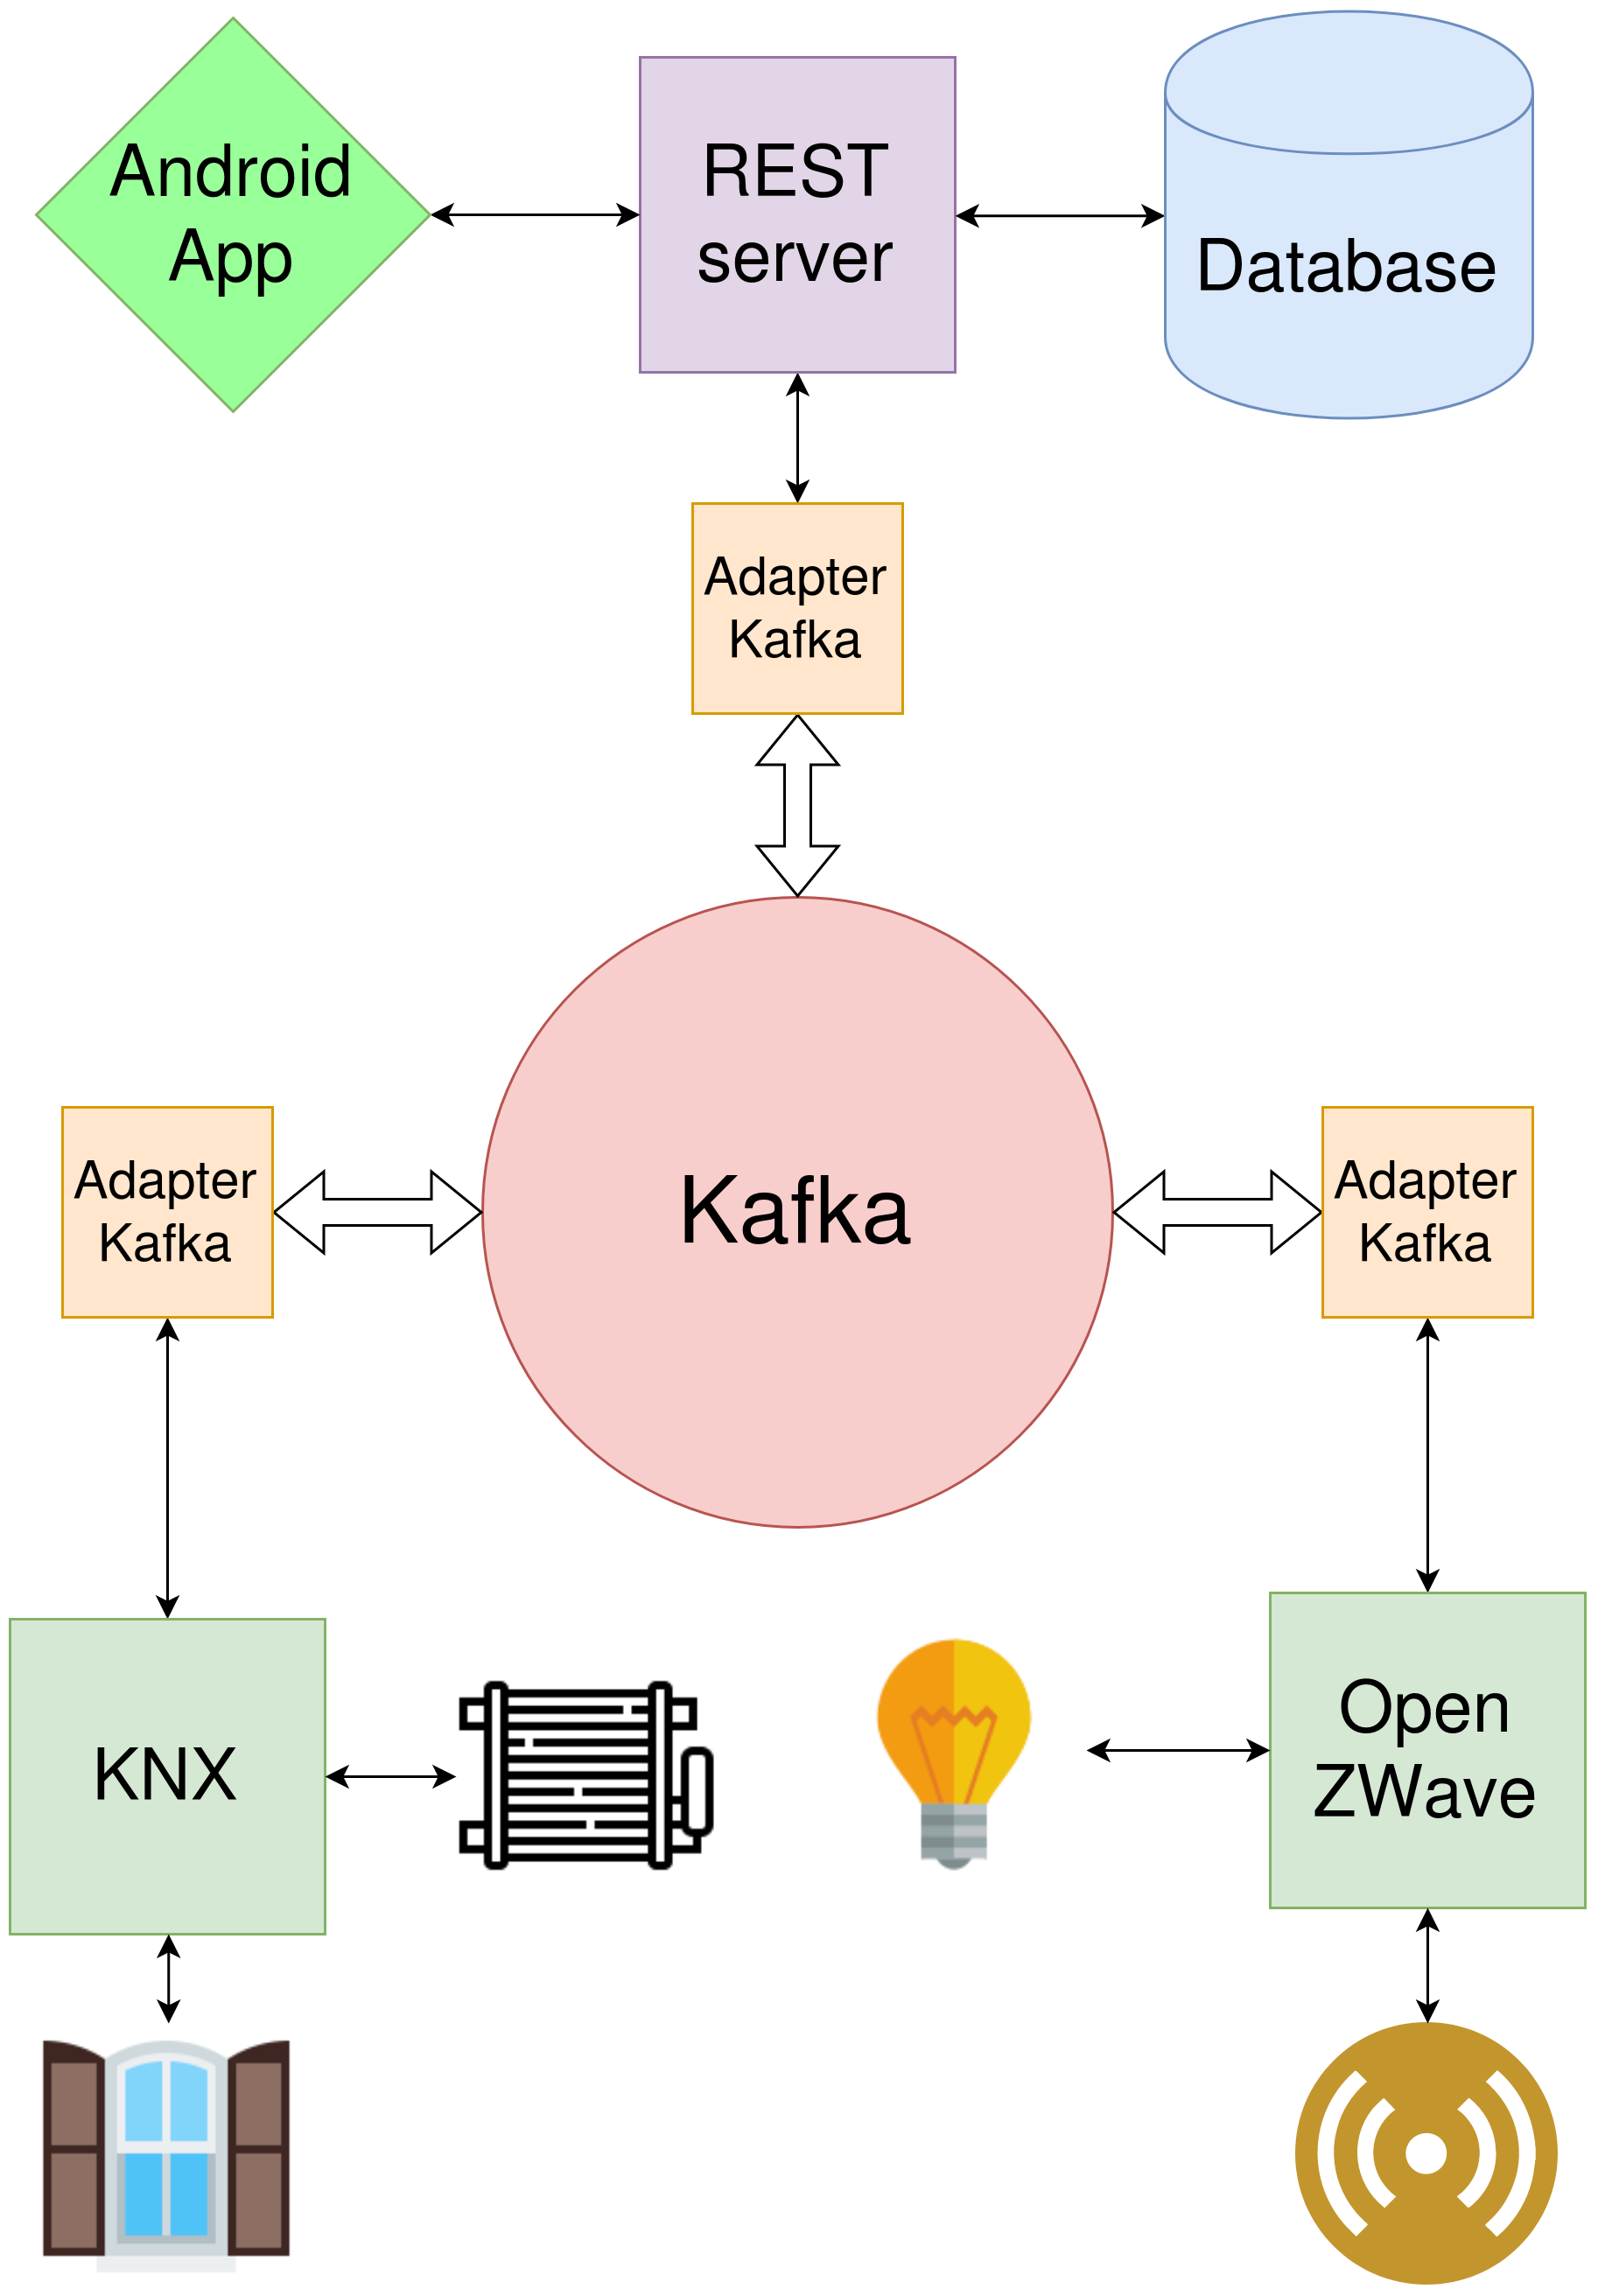
\includegraphics[width=0.8\textwidth]{img/general.png}
    \end{center}
    \caption{Architecture globale du système}
    \label{shema_general}
\end{figure}
